\documentclass[10pt, letterpaper]{article}
\usepackage{graphicx}




\usepackage[bottom=1.0in]{geometry}
\topmargin=-0.9in
\oddsidemargin -.3in
\evensidemargin -0.3in
\textwidth=7.0in
%\itemsep= -0.5in
%\parsep= -0.04in

\usepackage[cmex10]{amsmath}

\usepackage{color, colortbl}
\definecolor{Blu}{rgb}{0.4,0.4,1}


\makeatletter
\def\@seccntformat#1{%
  \expandafter\ifx\csname c@#1\endcsname\c@section\else
  \csname the#1\endcsname\quad
  \fi}
\makeatother



\author{Madhusudan Govindraju}
\date{}
\begin{document}
\title{Biometric Identification}
\maketitle

\section{Face Recognition using Eigenfaces}


\subsection{Find the Eigen Faces for corresponding top 10 eigen-vectors}
\begin{enumerate}
\item The face images are loaded from the data sets and rearranged to form a vector of size 2500xM where M is the number of images. Each image was originally 50x50 which has been rearranges to a one dimensional vector 2500x1, This is $\Gamma$
\item Find the mean image $\Psi$
\item Subtract the mean image from every image to get the $\Phi(i)$ and we group all the $\Phi(i....m)$ together to get the matrix A.
\item Now if we find the covariance of A to find the eigenvectors and eigenvalues . The resulting matrix is very large, instead of finding the covariance matrix $ A \times A^{T} $ we find the matrix $ A^{T}\times A $ and  then compute the eigenvectors($v_{i}$) 
$$
        A^{T}Av_{i} = \mu_{i}v_{i}	
$$
\item We sort the eigenvalues($\mu$) in descending order and then pick the top 10 eigenvectors corresponding to the top 10 eigenvalues, and calculate the eigenvectors$u_{i}$ of the $AA^{T}$ matrix using the following formula,
$$
u_{i} = Av_{i}
$$
\item This $u_{i}$ vector is rearranged in a $50\times50$ matrix to get the eigenfaces. 
\item The weights can be calculated by multiplying the top N required eigenfaces with the matrix $A$.
\end{enumerate}

\subsection{Compute the eigen-coeff for top 30 eigen-faces}

\begin{enumerate}
\item From the sorted vector containing the eigenvalues the top 30's corresponding {\sl eigenvectors} are chosen. 
\item Calculate the eigenvectors of $AA^{T}$ with the formula $u_{i} = Av_{i}$. 
\item The weights of the gallery images can be obtained from  $u_{i}$ with the formula $u_{i}^{T} \times A $. The weights for the probe images can be obtained using from $u_{i}$ with the formula $u_{i}^{T} \times A_{probe} $.
\item We find the distance measure between these two weights to get the similarity matrix for the face recognition purpose.

\end{enumerate}

\subsection{ ROC, CMC, Genuine and Imposter Disribution, Rank-1 Identification Curve}

The above mentioned graphs are plotted for different coefficients taken from 30 to 100 in steps of 10. They can be found in the later sections of this report with appropriate headings. From the graphs it can be understood that increasing the number of coefficients do not have and effect on the performance of the system. This can be verified easily from figures \ref{fig:Rank1Eu} \ref{fig:Rank1Cheby} \ref{fig:Rank1Min} \ref{fig:Rank1CB}.

\subsection{Distance measures}
Four different distance measures are used in this assignment they are \\
Eucledian Distance :   $ d_{st} =  \sqrt{  (x_{2} - x_{1})^2 + (y_{2} - y_{1})^2  }  $ \\
Chebychev Distance :  $ d_{st} = max_{j} \{ |x_{sj}  - x_{tj} | \}  $ \\
Minkowski Distance :  $    d_{st} = \sqrt[p]{ \Sigma_{j=1}^{n} |x_{sj} - x_{tj}|^{p} }    $\\
City Block Distance : $   d_{st} = \Sigma_{j=1}^{n} |x_{sj} - x_{tj}|     $  \\


Among these City - Block Distance measure seems to work the best having the rate at 85\% and the worst distance measure would be chebyshev performing at 59\% . The Distance measure in the order of performance is City-Block ,Euclidean, Minkowski, Chebyshev.

\begin{figure}
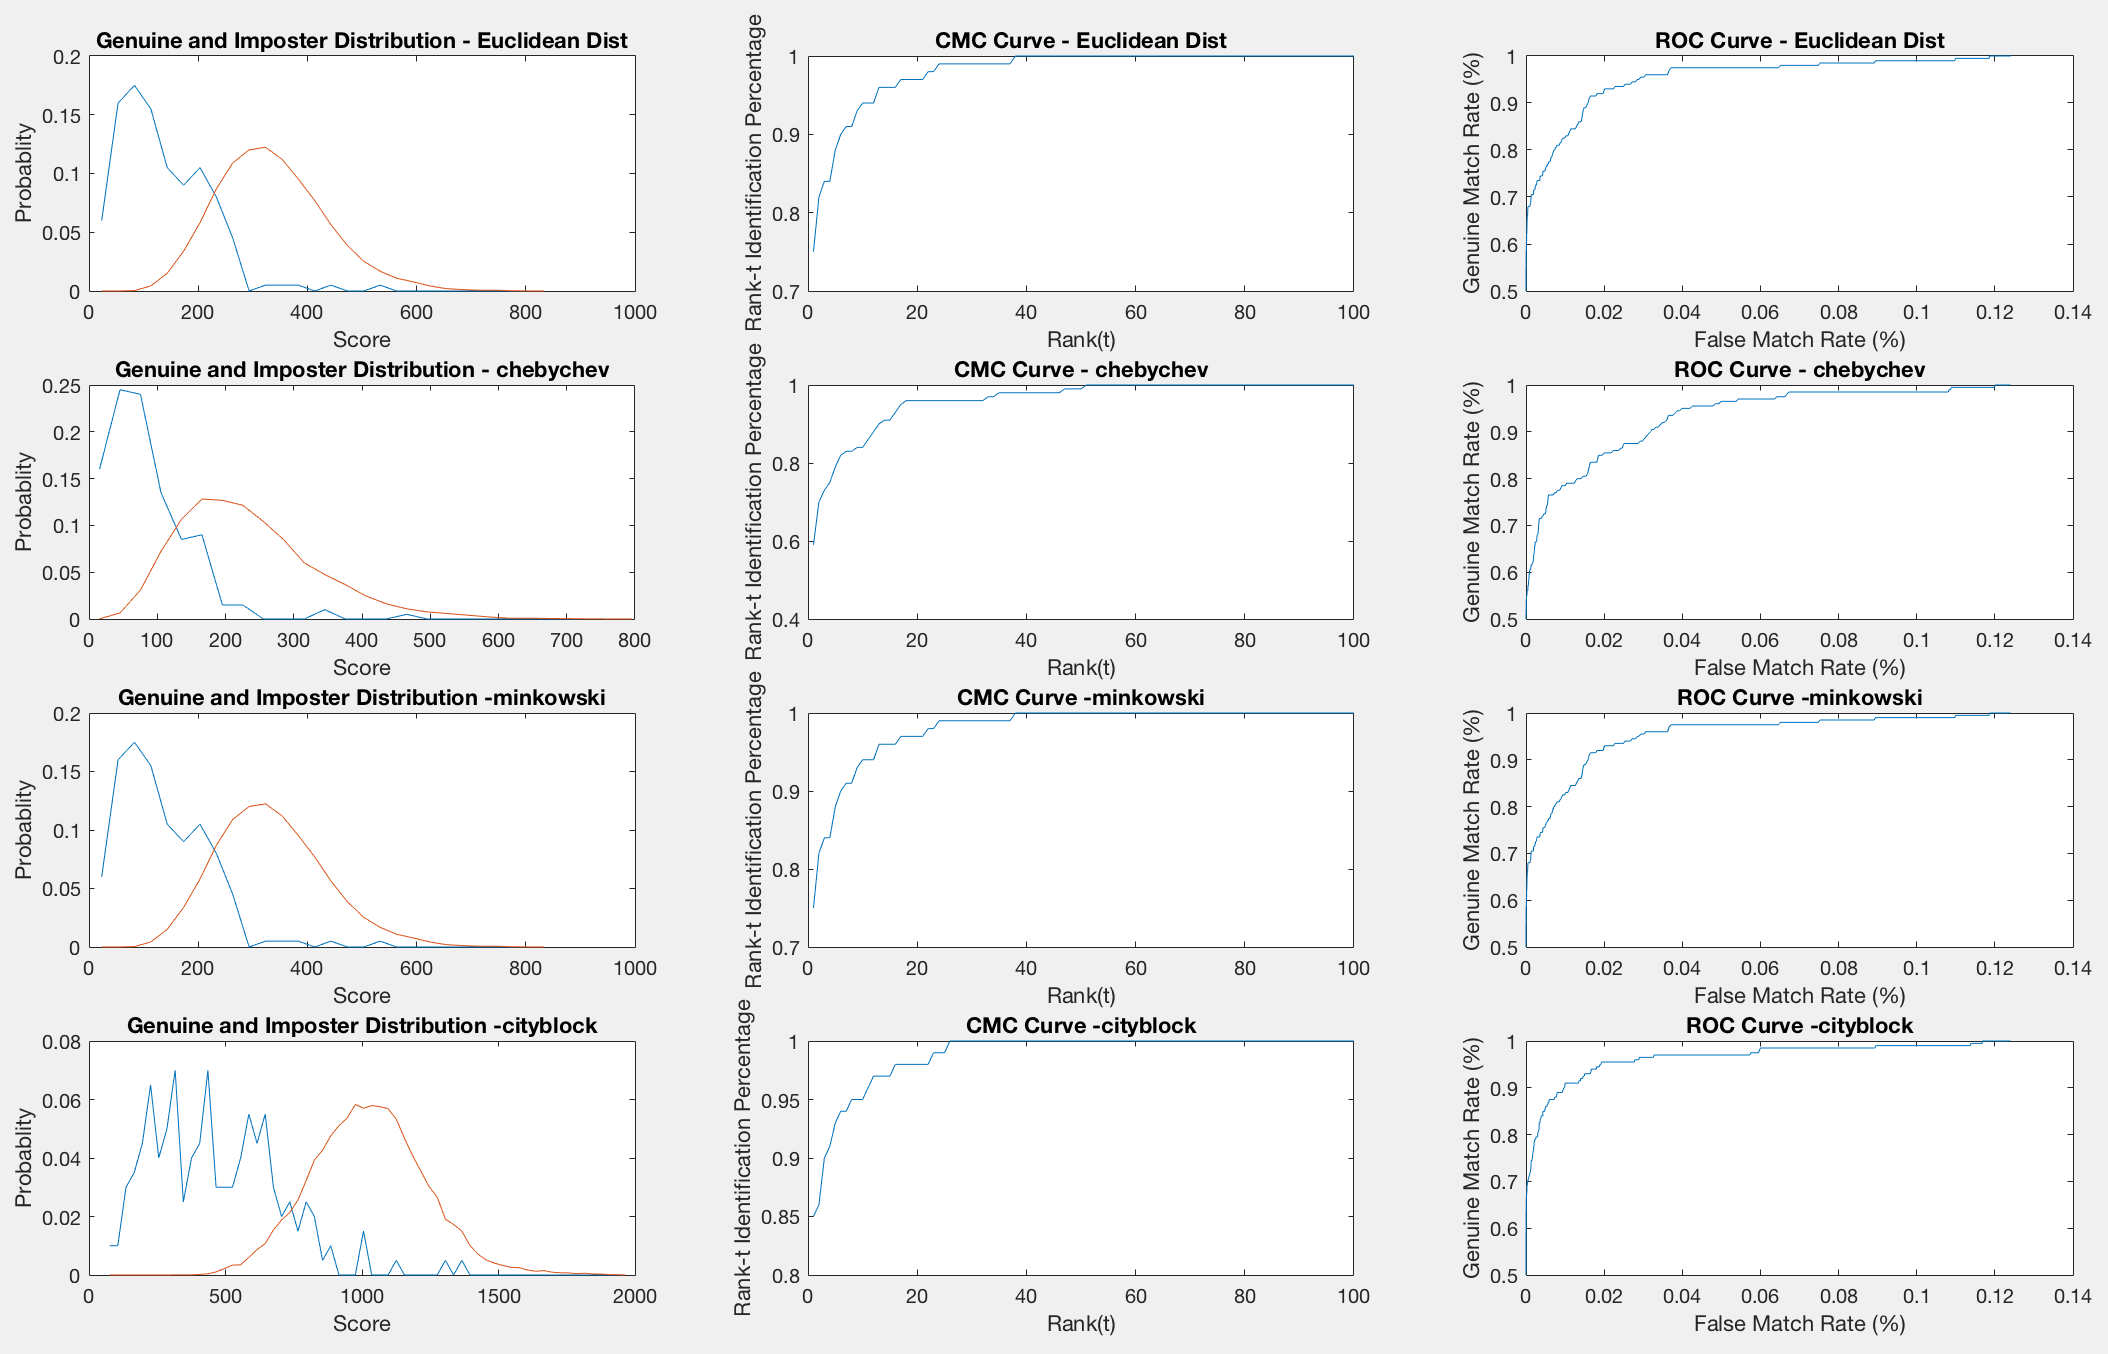
\includegraphics[width=\linewidth]{images/for30coeff}
 \caption{ Plots for 30 Eigenvectors}
 \label{fig:30coeff}
 
 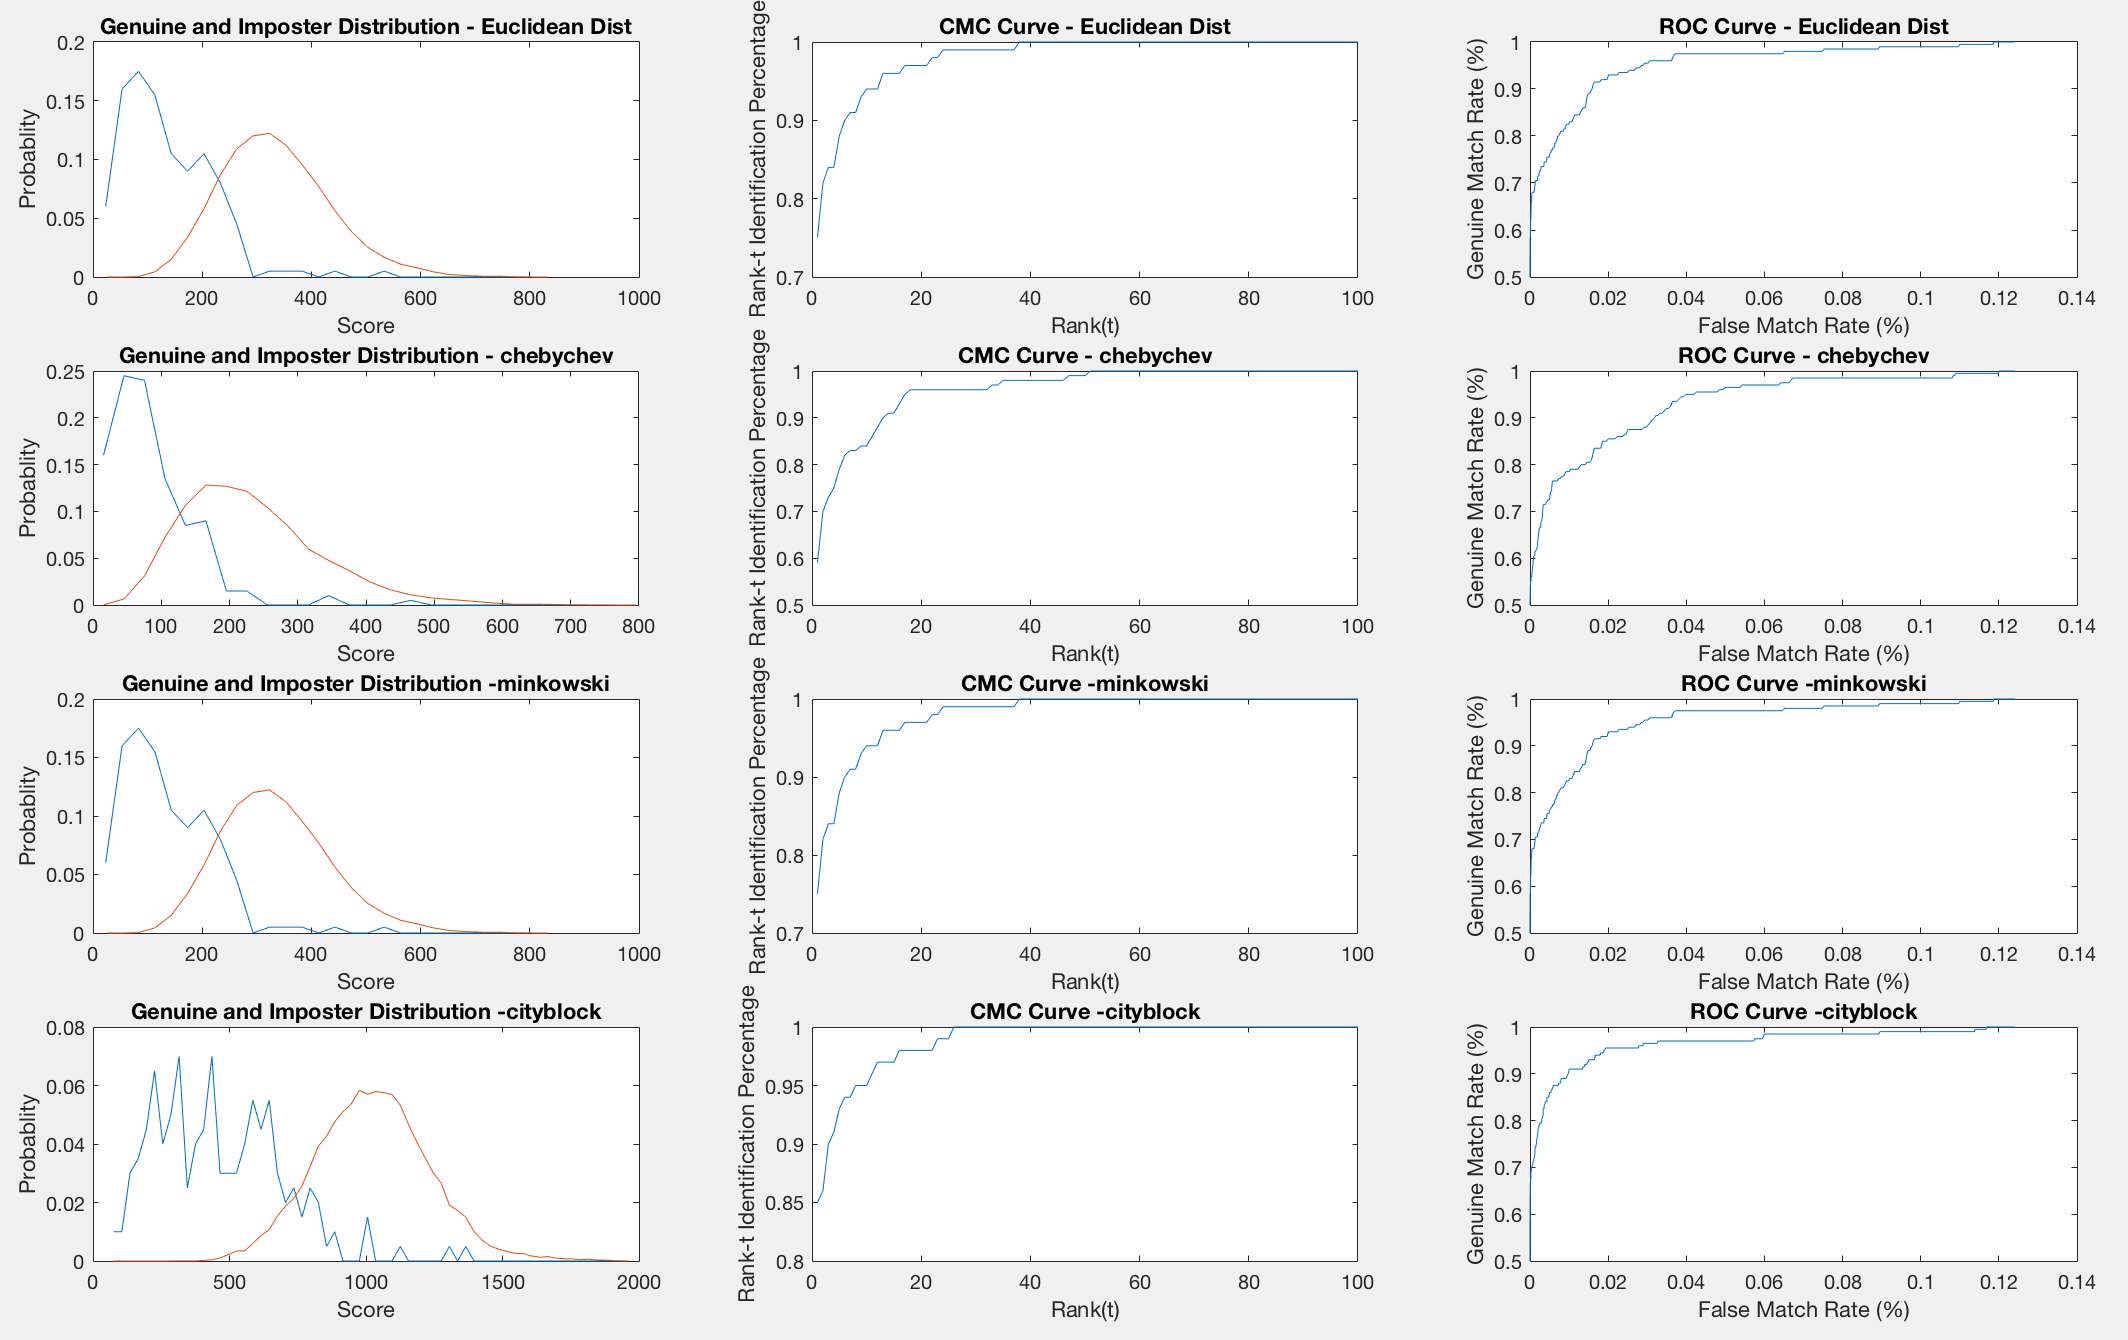
\includegraphics[width=\linewidth]{images/for40coeff}
 \caption{ Plots for 40 Eigenvectors}
 \label{fig:40coeff}
  
\end{figure}
\begin{figure}
 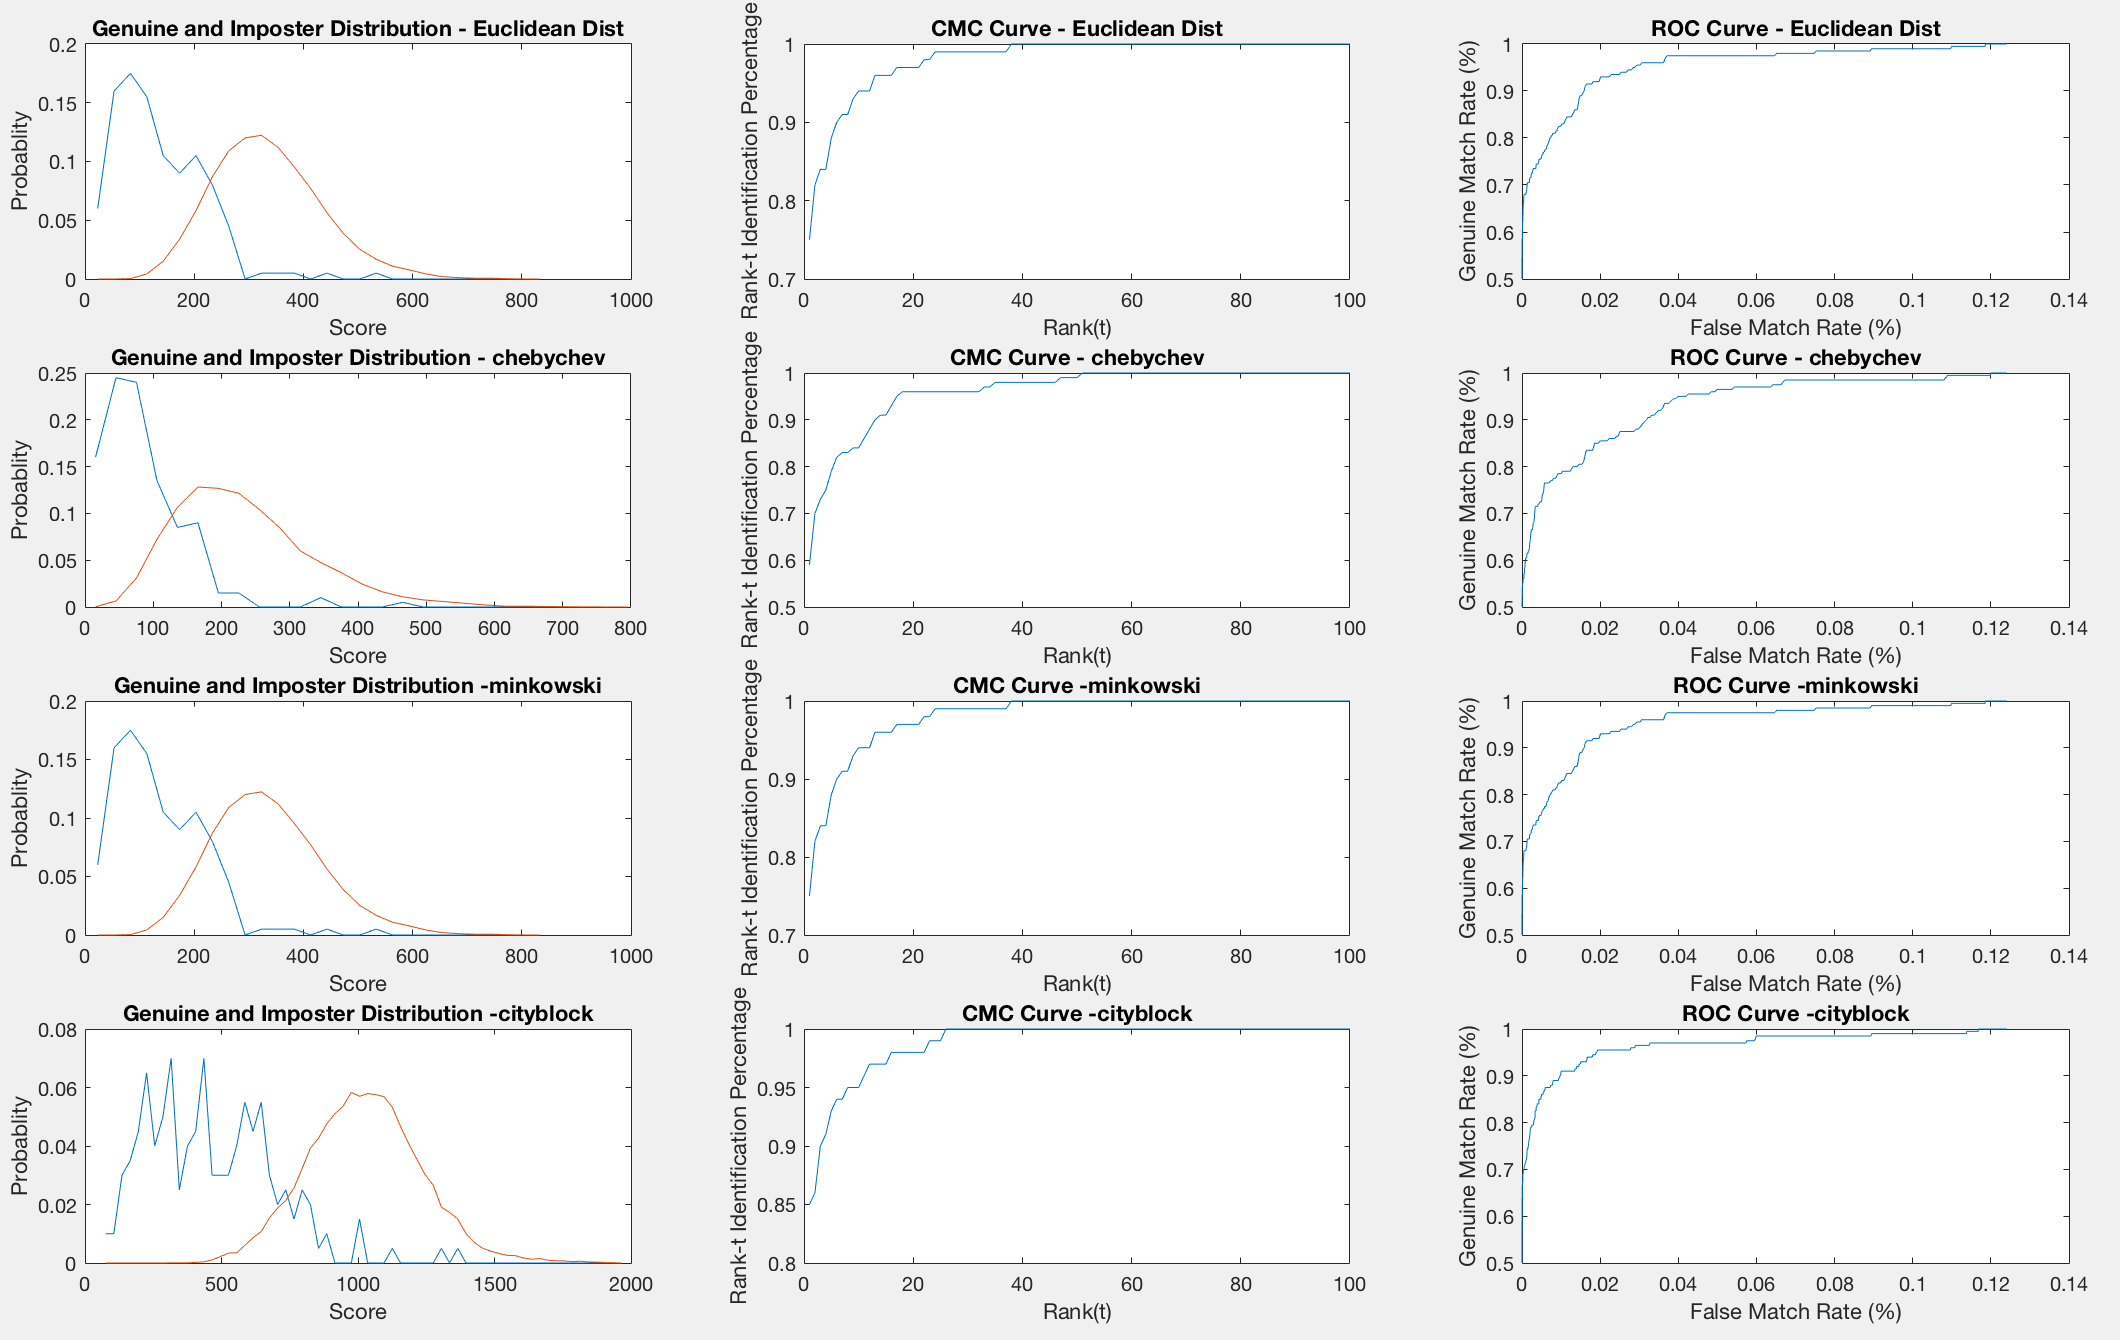
\includegraphics[width=\linewidth]{images/for50coeff}
 \caption{ Plots for 50 Eigenvectors}
 \label{fig:50coeff}

  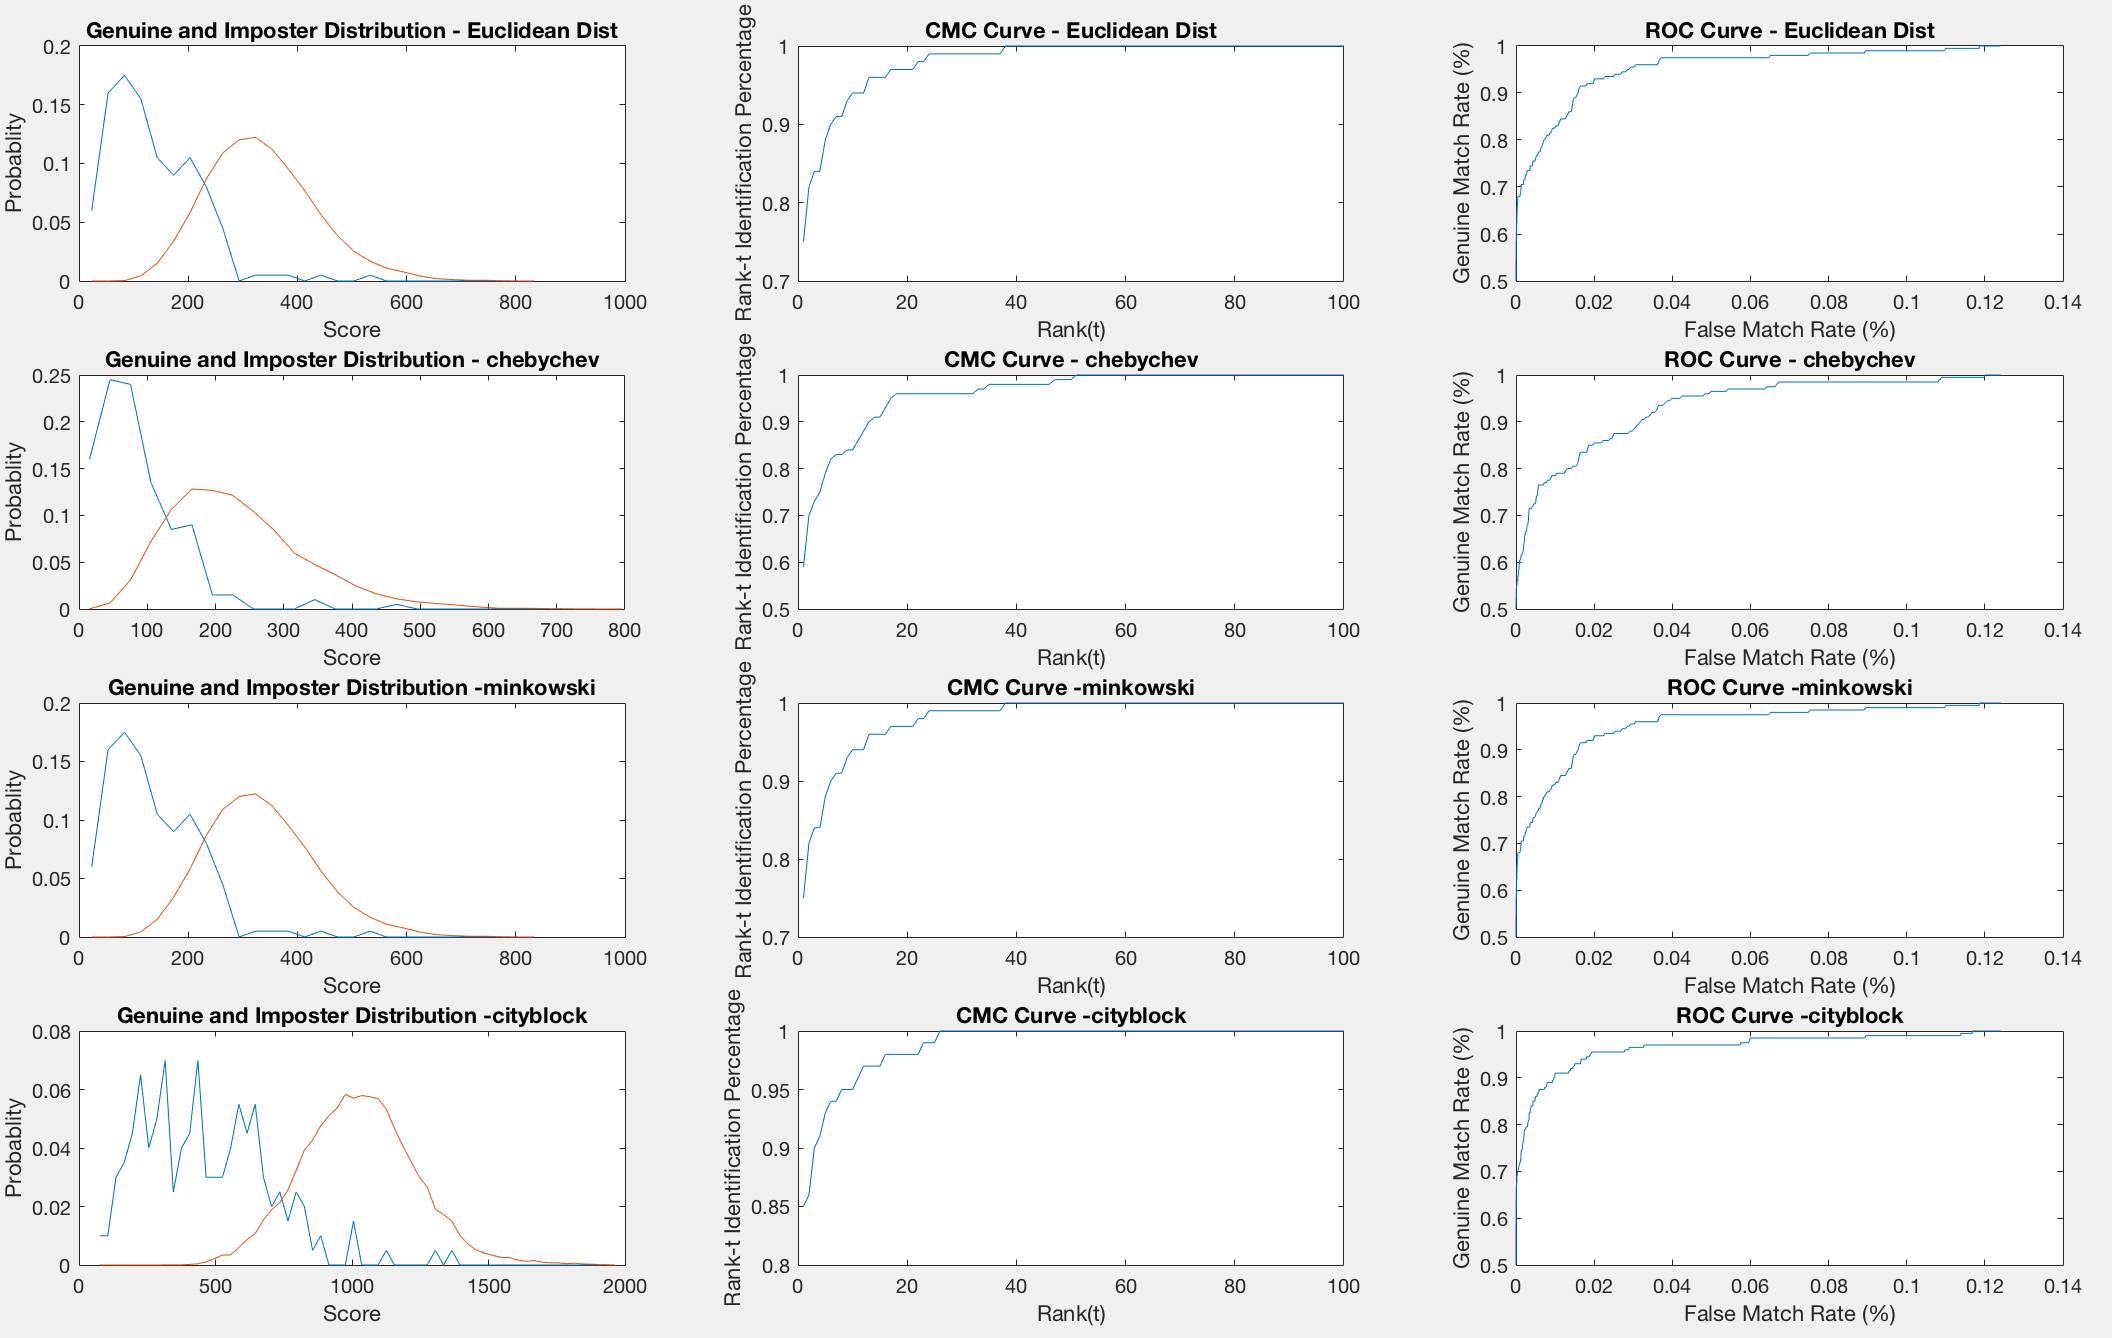
\includegraphics[width=\linewidth]{images/for60coeff}
 \caption{ Plots for 60 Eigenvectors}
 \label{fig:60coeff}
\end{figure}

\begin{figure}
   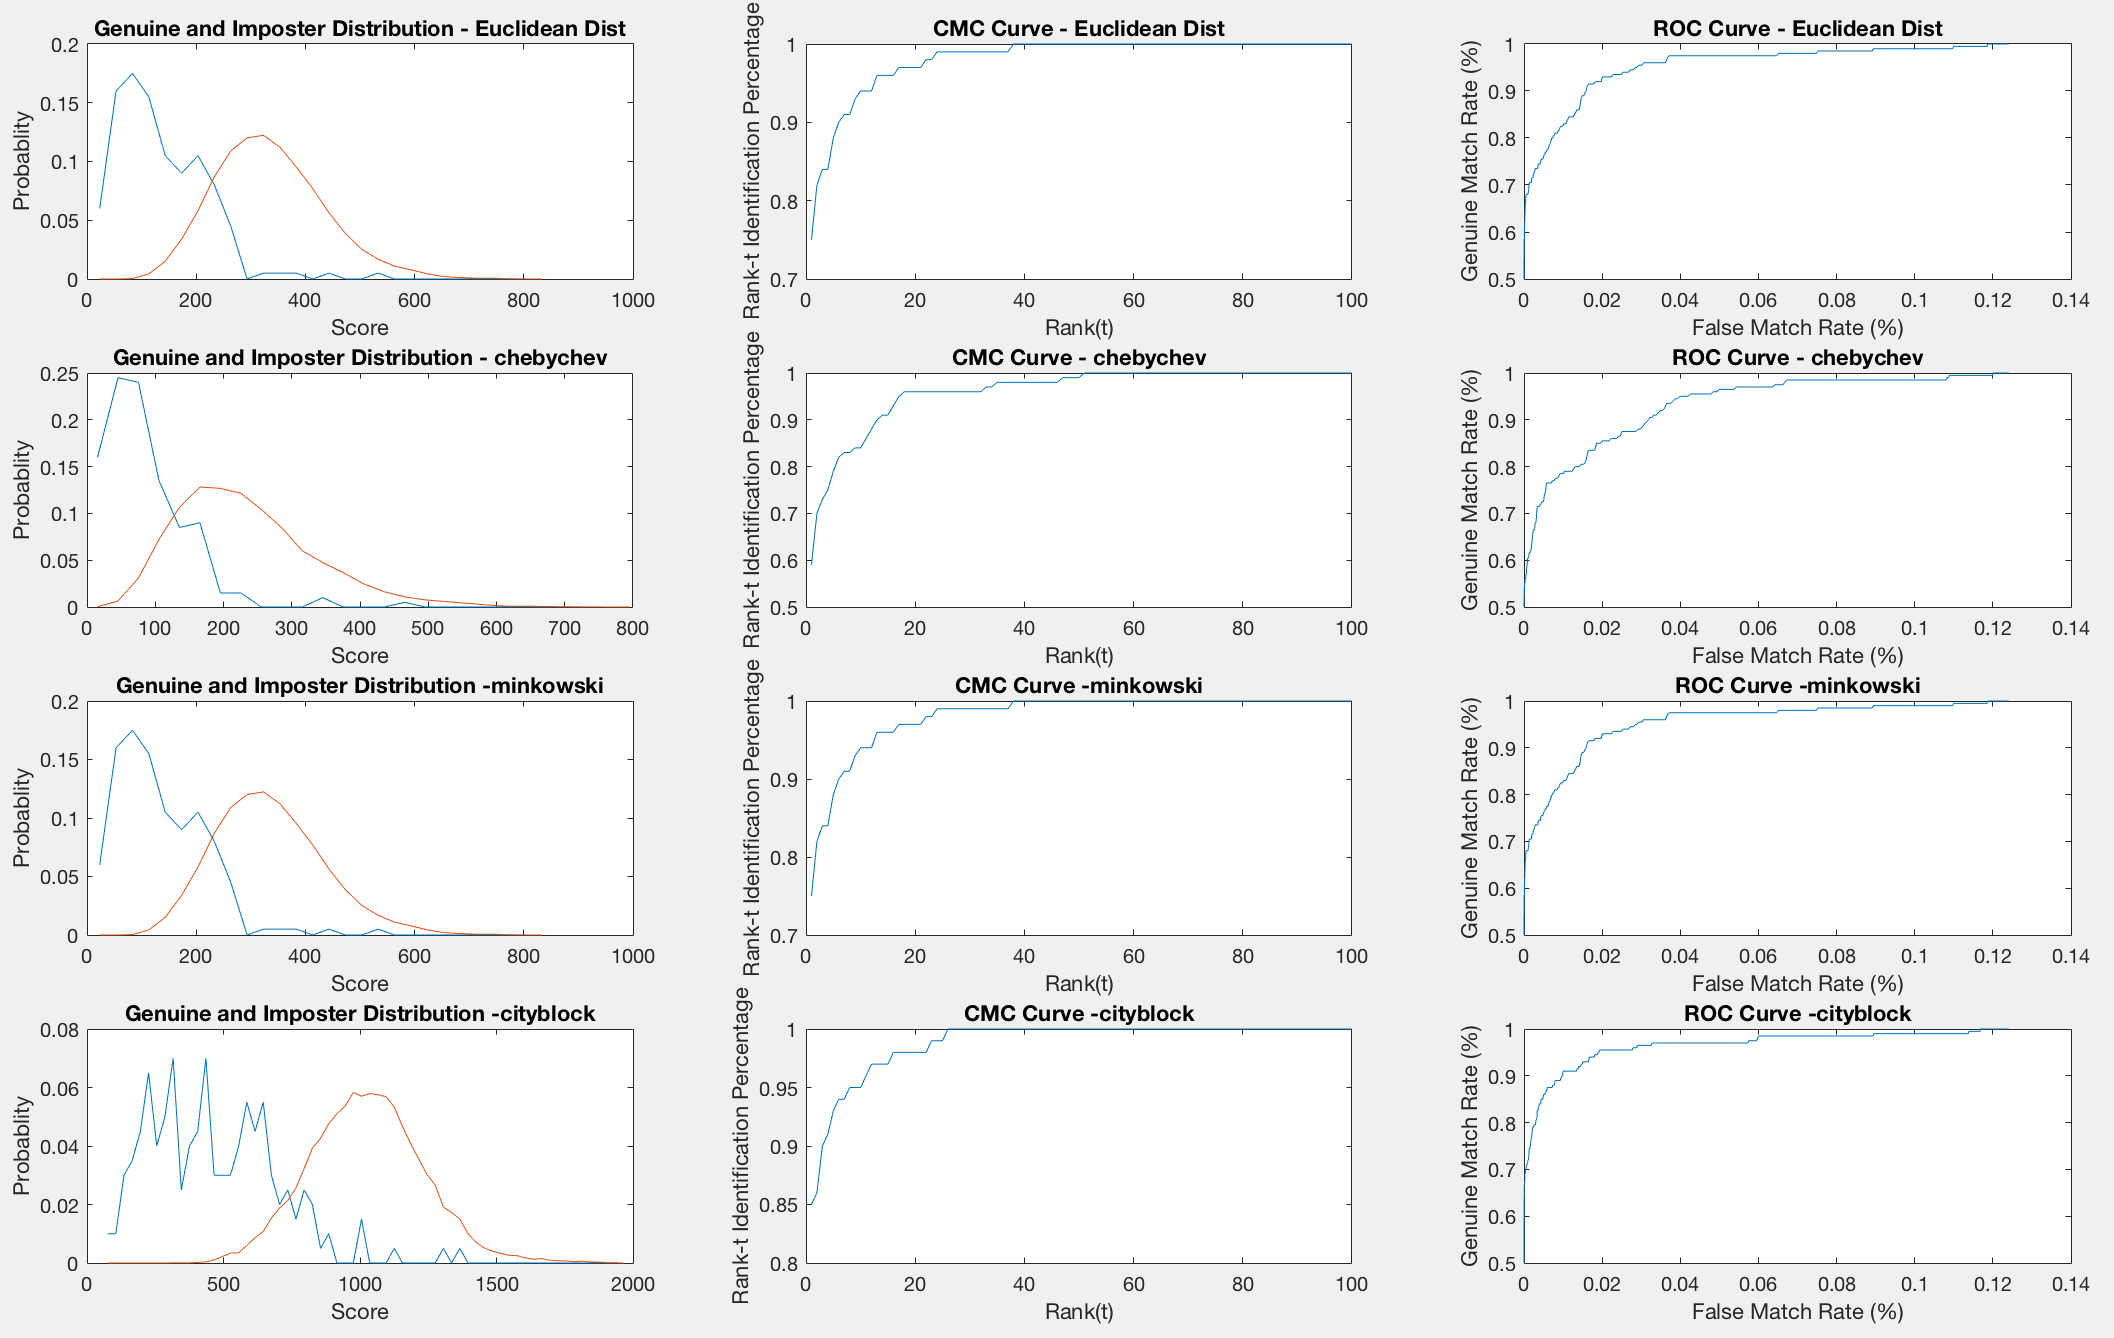
\includegraphics[width=\linewidth]{images/for70coeff}
 \caption{ Plots for 70 Eigenvectors}
 \label{fig:70coeff}
 
   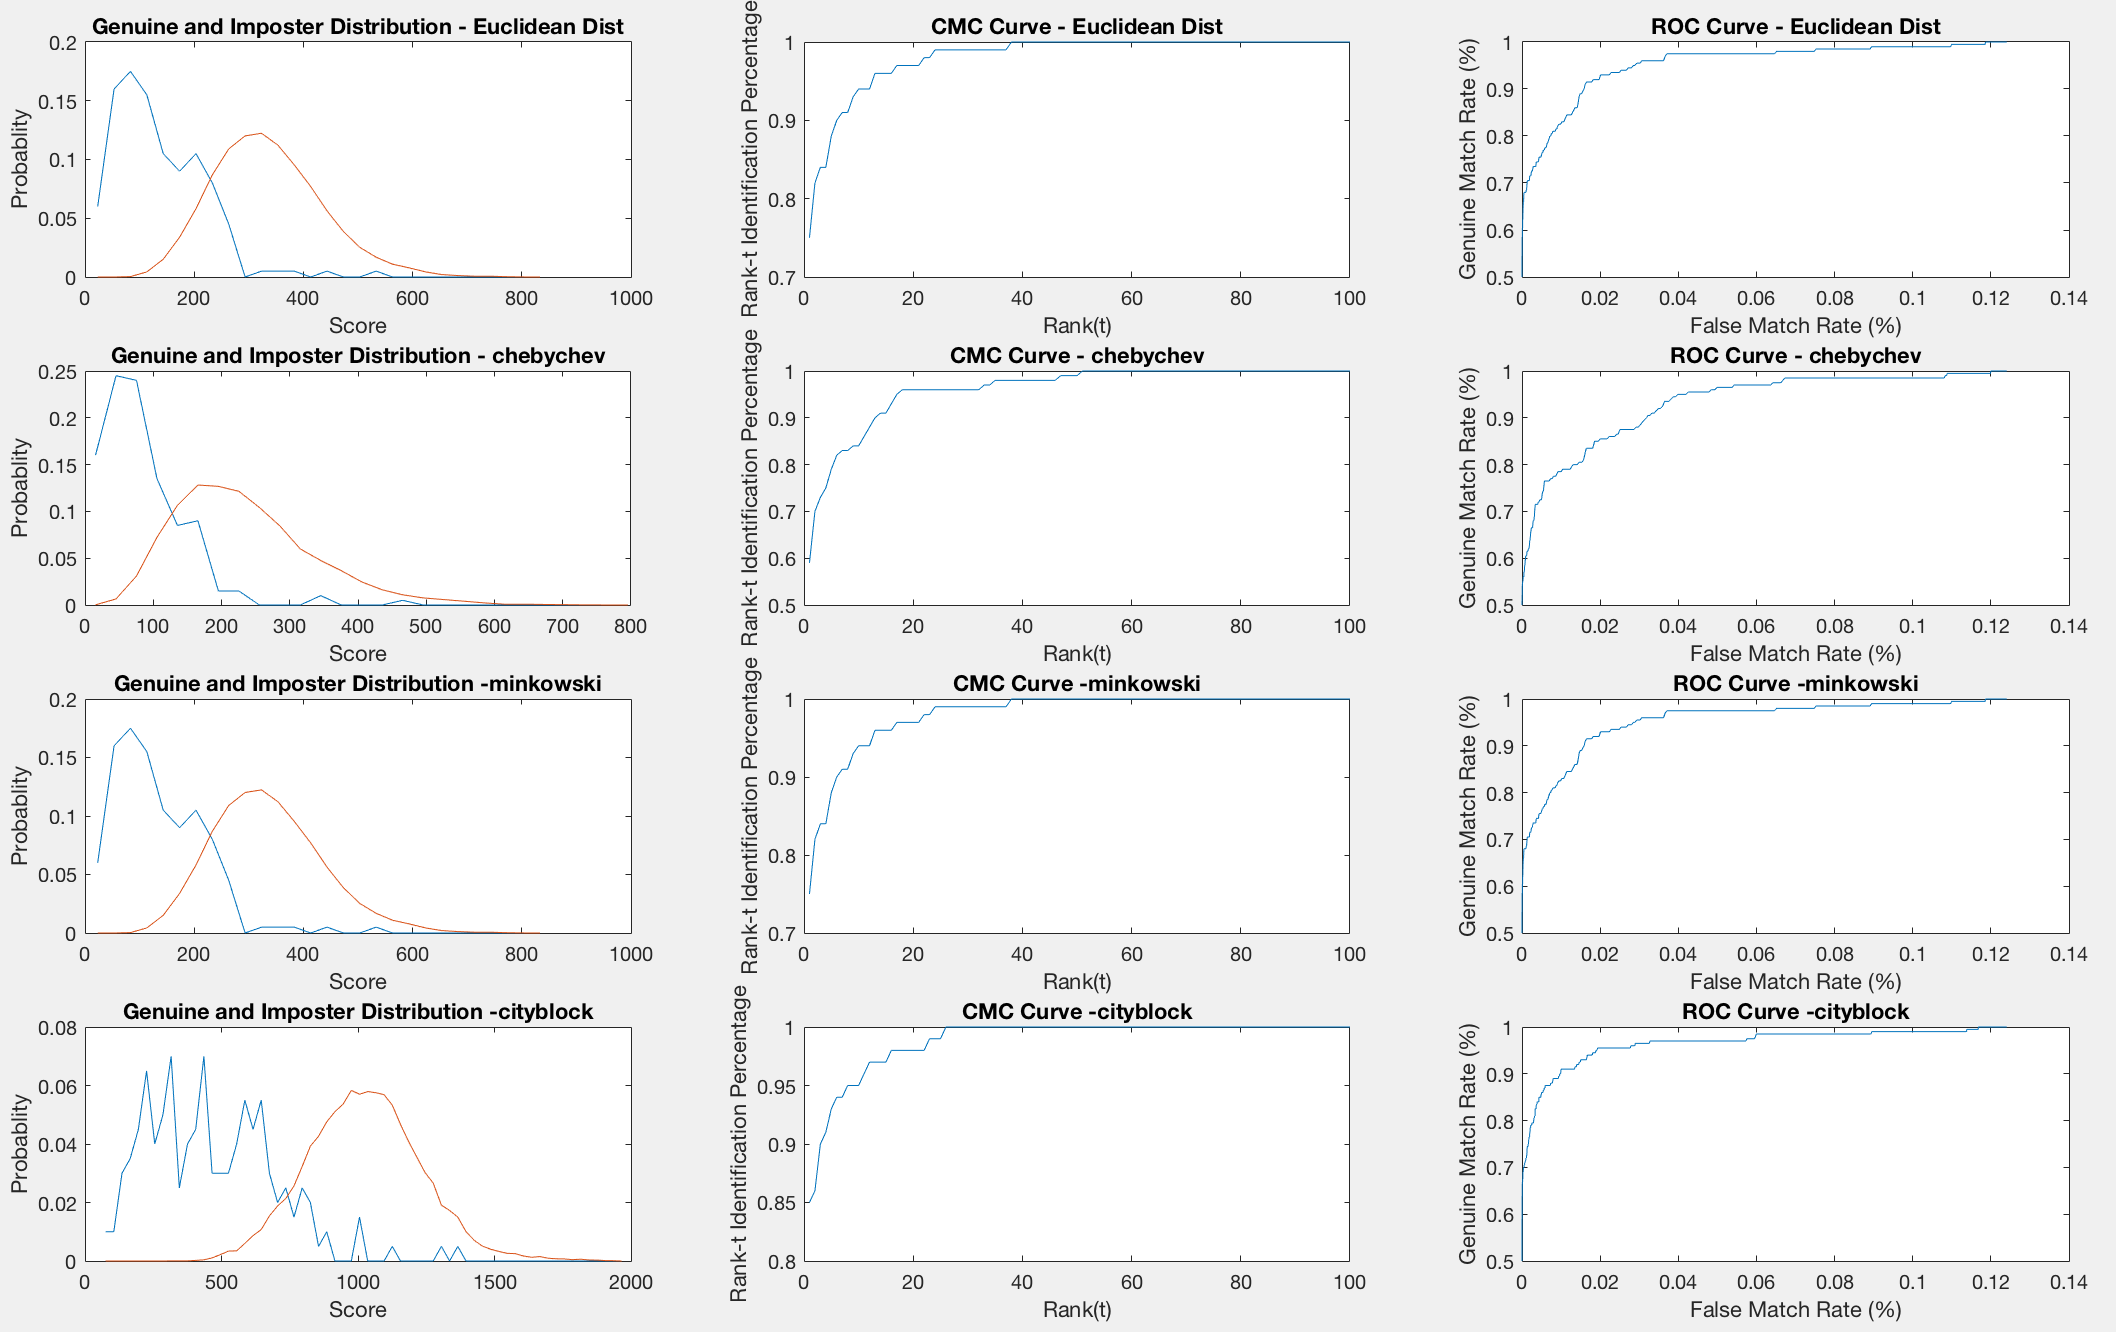
\includegraphics[width=\linewidth]{images/for80coeff}
 \caption{ Plots for 80 Eigenvectors}
 \label{fig:80coeff}
\end{figure}

\begin{figure}
    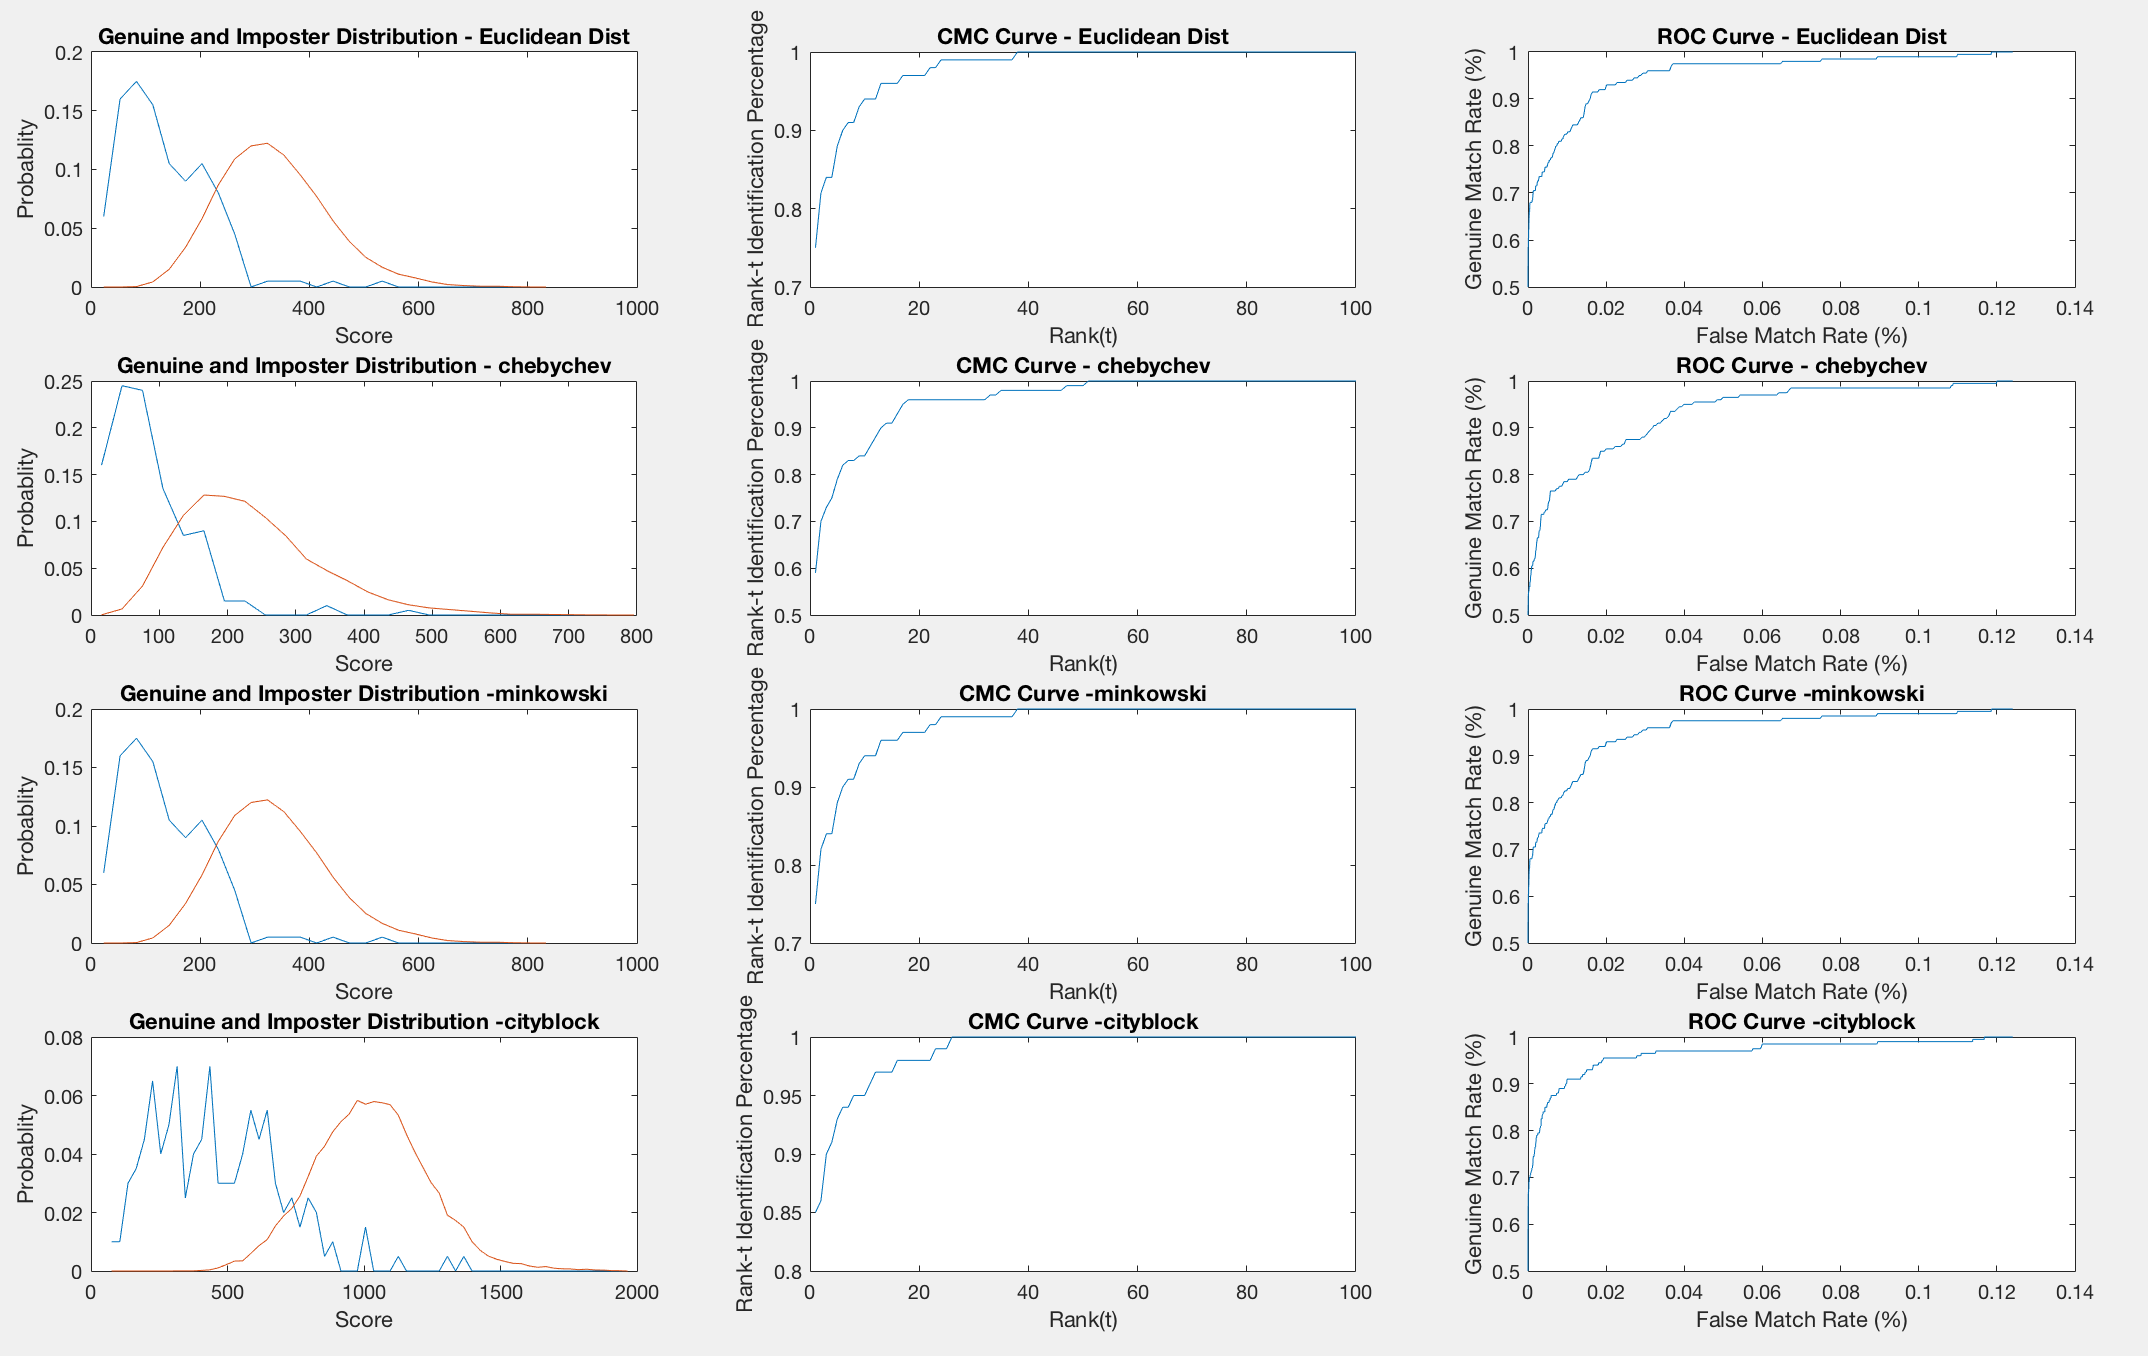
\includegraphics[width=\linewidth]{images/for90coeff}
 \caption{ Plots for 90 Eigenvectors}
 \label{fig:90coeff}
 
     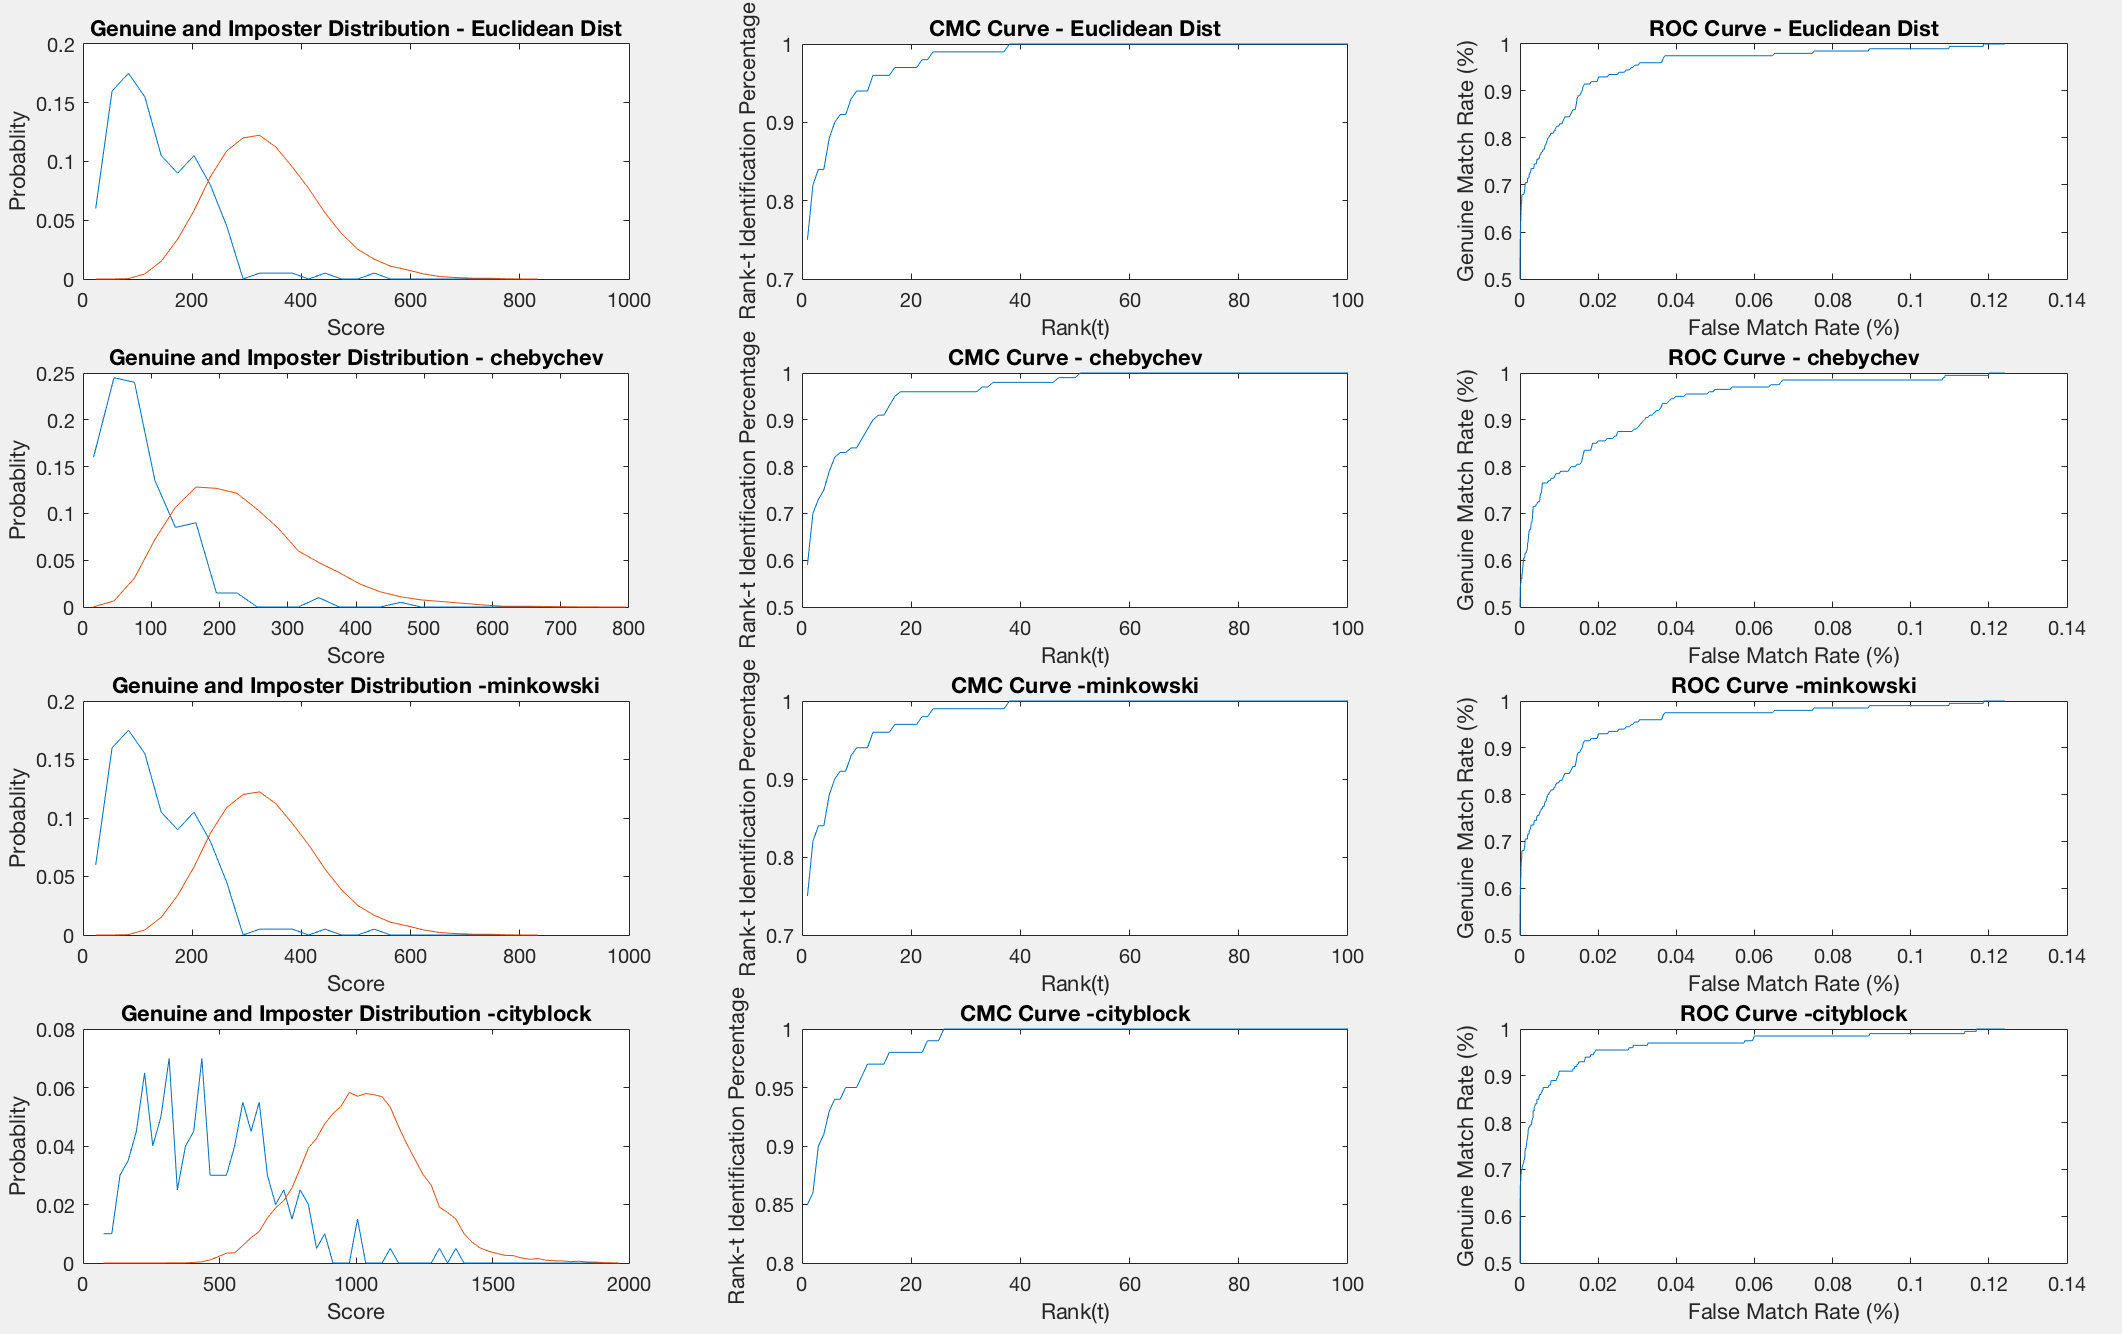
\includegraphics[width=\linewidth]{images/for100coeff}
 \caption{ Plots for 100 Eigenvectors}
 \label{fig:100coeff}
\end{figure}

\begin{figure}
    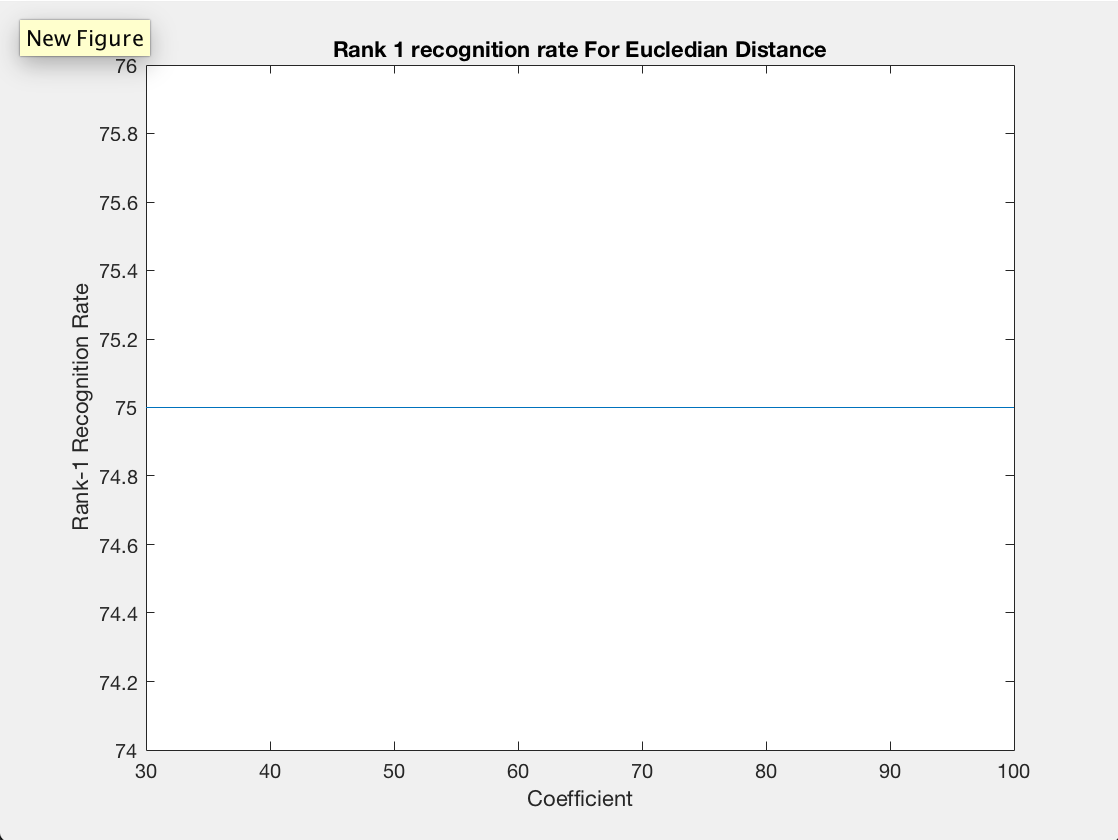
\includegraphics[width=\linewidth]{images/Rank1Rate_Euclidean}
 \caption{ Rank 1 Recognition rate for Euclidean Distance}
 \label{fig:Rank1Eu}
\end{figure}

\begin{figure}
    \includegraphics[width=\linewidth]{images/Rank1Rate_Chebychev}
 \caption{ Rank 1 Recognition rate for Chebychev Distance}
 \label{fig:Rank1Cheby}
\end{figure}

\begin{figure}
    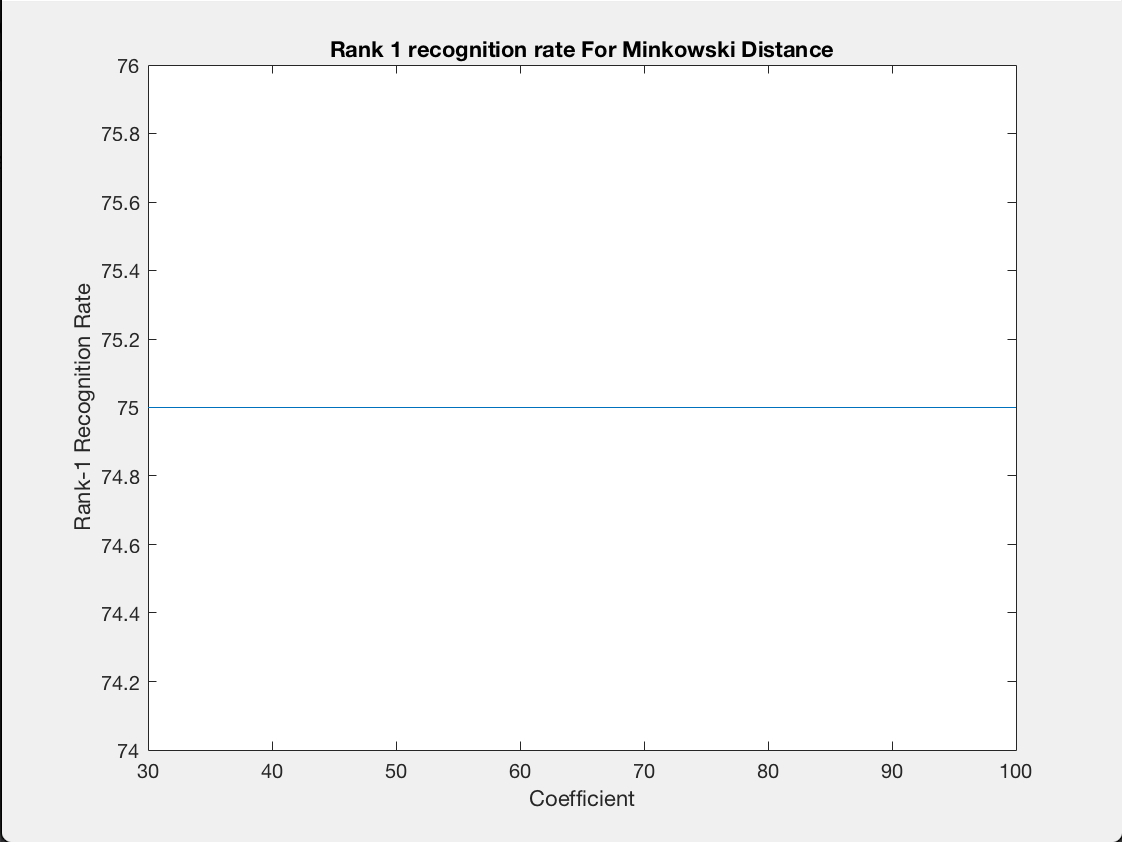
\includegraphics[width=\linewidth]{images/Rank1Rate_Minkowski}
 \caption{ Rank 1 Recognition rate for Minkowski Distance}
 \label{fig:Rank1Min}
\end{figure}

\begin{figure}
    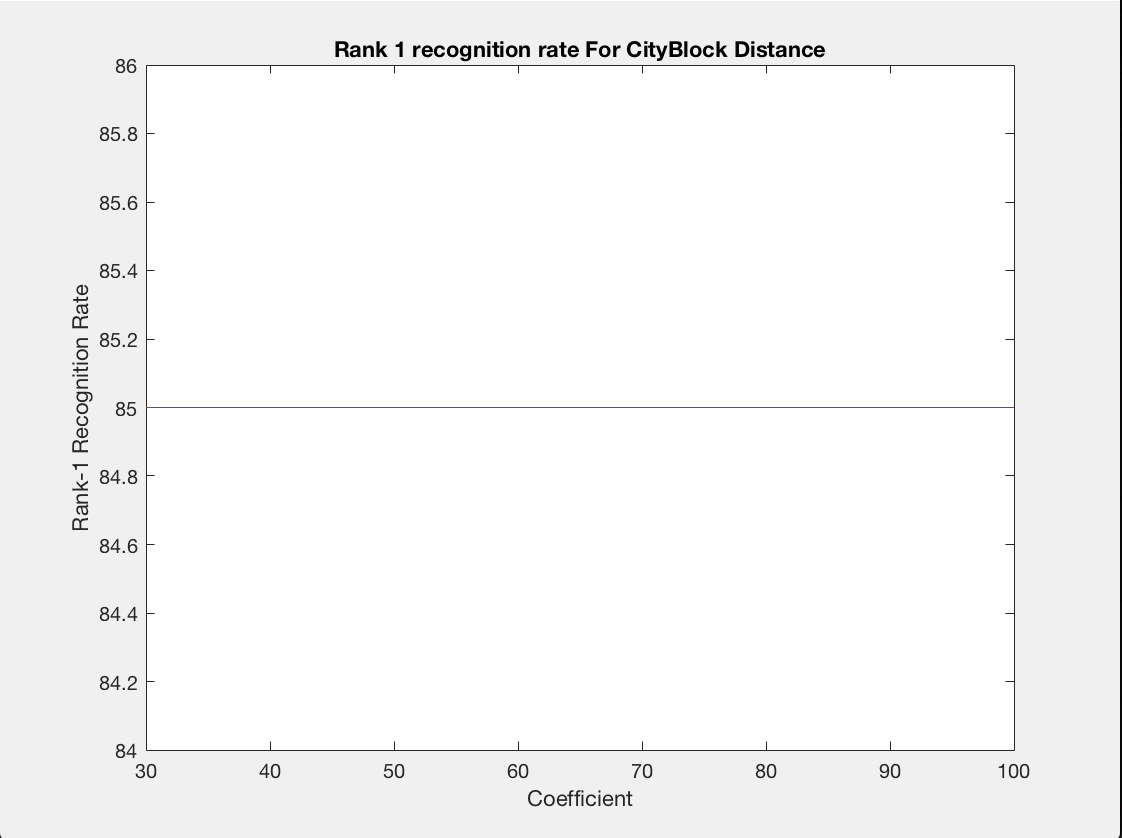
\includegraphics[width=\linewidth]{images/Rank1Rate_CityBlock}
 \caption{ Rank 1 Recognition rate for City Block Distance}
 \label{fig:Rank1CB}
\end{figure}



\end{document}